\documentclass[12pt]{article}

\usepackage[utf8]{inputenc}
\usepackage[T1]{fontenc}
\usepackage{amsmath}
\usepackage{hyperref}
\usepackage{graphicx}

\graphicspath{{images/}}
\hypersetup{colorlinks=true, citecolor=blue}

\begin{document}

\title{Toward Controlled Generation of Text}
\author{}
\date{}
\maketitle

\section{Idea}
  The authors aim to disentangle representations of style and content in the latent code of an Adversarial Variational AutoEncoder. The style is called the \textbf{structured code} and is learned by discriminators for each attribute that needs to be disentangled from the latent space.

\section{Method}
  \begin{itemize}
    \item This method does not use adversarial training.
    \item The basic approach can be described as below:
    \begin{itemize}
      \item $x$ is the source corpus
      \item The encoder is parameterized to generate a latent code $z$, which is a variational latent space that resembles a Gaussian prior. (This is enforced by a KL-divergence loss)
      \item The structured code $c$ is a known label of the text (discrete or continouous)
      \item The decoder generator produces the output corpus $\hat{x}$ conditioned on $(z, c)$. It uses greedy decoding.
      \item A classifier/regressor discriminator predicts the structured code of the output corpus $\hat{x}$ to ensure that it is the same as the one the generator was conditioned on i.e. $G(z, c)$. The discriminator is pretrained.
      \item Each decoder step in $\hat{x}$ is predicted using a softmax function scaled by a temperature $\tau$. Higher temperatures flatten the softmax distribution for each word prediction and increase word diversity. Conversely, setting $\tau = 0$ will resembled a hardmax. For their experiments the authors gradually anneal $\tau \rightarrow 0$
    \end{itemize}
    \item The authors describe 3 separate losses to train their model.
    \begin{itemize}
      \item A reconstruction loss that ensures that the generated sentence $\hat{x}$ is the same as the original sentence $x$. This is equivalent to minimizing the negative log-likelihood of generating $\hat{x}$.
      \item A discriminator validates if the predicted class/value for $\hat{x}$ is the same as the corresponding class/value for $x$. This is a cross-entropy loss over the probability distribution of the labels. This discriminator loss can be further subdivided into 2 terms.
      \begin{itemize}
        \item Maximize the expected log likelihood of predicting the correct distribution of the structured code $c$ given the labelled examples $X_L$. This happens before the generator model training.
        \item Maximize the expected log likelihood of predicting the correct distribution of the structured code $c$ given the generated sentences $\hat{x}$. Also minimize the empirically observed Shannon entropy of the observed discriminator prediction $q_D(c\prime|\hat{x})$, which reduces uncertainty and increases confidence of the structured code prediction.
      \end{itemize}
      \item The encoder from loss 1, is used to regenerate the latent distribution $z$ devoid of the structured code from the output distribution $\hat{x}$. The authors call this an \textbf{independence constraint}, in that regardless of the structured code $c$ that is currently present in either $x$ or $\hat{x}$, processing either through the generator should produce a consistent $z$. This allows the encoder to encode only latent factors that are independent of the structured code.
    \end{itemize}
    \item A wake-sleep algorithm \cite{hinton1995wake} is used to alternatively train the generator and discriminator.
    \item The model was applied only to short sentences with length $<15$ words.
    \item The encoder/decoder setup is implemented using single layer LSTMs and the discriminator is implemented using conv-net. The KL term is annealed from 0 to 1 during training.
  \end{itemize}

\section{Architecture}
  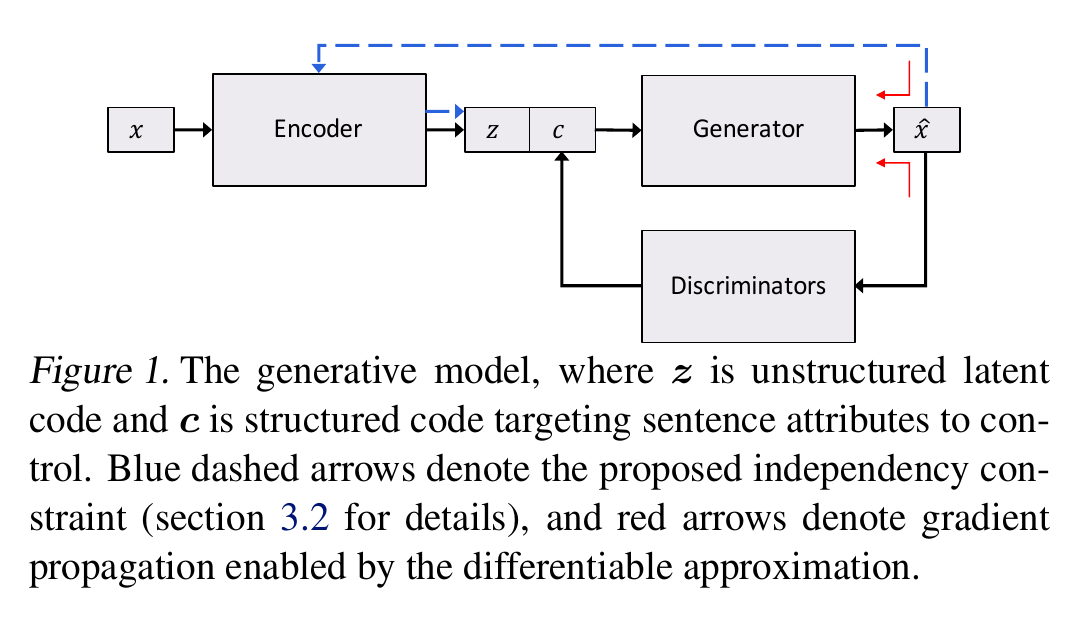
\includegraphics[width=\textwidth]{architecture}

\section{Learning Process}
  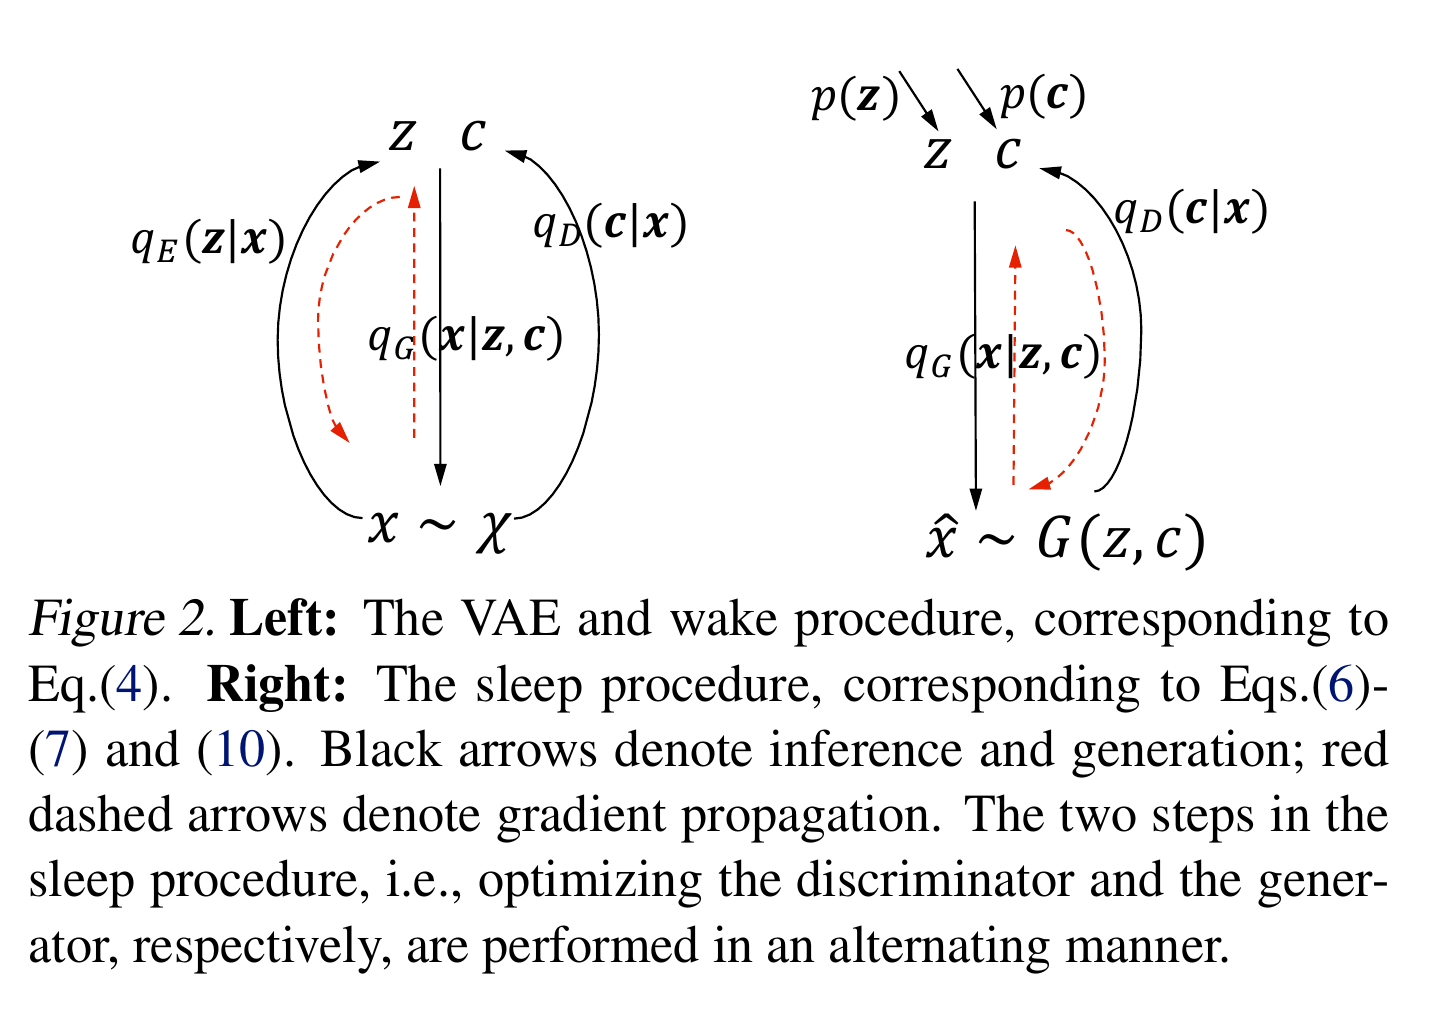
\includegraphics[width=\textwidth]{learning-process}

\section{Observations}
  \begin{itemize}
    \item The model performs better than the S-VAE \cite{kingma2014semi} implementation in terms of sentiment accuracy of generated sentences.
    \item From the reported results, it seems that adding the independence constraint helps the generated sentences retain the content successfully.
  \end{itemize}

\bibliographystyle{unsrt}
\bibliography{toward-controlled-generation-of-text}

\end{document}
